Looking at design frameworks and elements with the goal to engage and capture their players from games in general and gamification as well as the connections between game elements and principles for engaged and effective learning show a lot of cross-over and allow for compilation into overarching aspects and game design elements that many authors seem to agree to be the key to sucessful game development for commercial games and gamification applications alike.

\textbf{Fantasy} or \textbf{Game Fantasy} is one of such core game elements, comprising not only the imagination of the player, but generally the scenario portrayed in the game material and the setting of it - refering to the environment that was built around the core mechanics of the game, giving it a believable context within the imaginary realm and help the player visualise it better \cite{aspects} \cite{model}. The knowledge that activity in the virtual space has no impact on the reality while the imaginary world captivates the player and makes them feel like nothing outside of it is relevant causes deeper engagement from the user, fostering interest in the activity and motivation to keep going, which increase the efficiency of learning environments through using this aspect within a gamified context \cite{aspects}.
It is important to note that despite the need for a convincing game fantasy, there has to exist a believable \textbf{relation to reality}. Games in their nature are often just enhanced simulations of real life activities, made more interesting by gamification techniques, but this is key in allowing the user to intuitively understand some ground rules about the world without needing a tiresome introduction \cite{lifelong} \cite{fail}.

Another important Game Element that is similar to and can go hand in hand with Game Fantasy is the \textbf{Narrative} within the game or gamified application. Briefly put, the game narrative is the description of happenings within the virtual space \cite{model}. Narrative Structures exist to provide immersion through storytelling within the game and allow the player to situate themselves within that world, enabling them to identify themselves better with the events that are happening as well as their player character \cite{lifelong}. Additionally, predictability is yet another aspect that a well thought out narrative structure may bring to the game, allowing the player to understand the imaginary world and it's machinations on a deeper level and learn to navigate it more intuitively. The gamified habit tracking and task management application Habitica (developed by HabitRPG, 2013) includes user oriented narrative through a role-playing game system, allowing the users to immerse themselves through the use of a personalised avatar and role-playing mechanics like a health bar and magic meter, as shown in Figure \ref{fig:3} \cite{avatar}.

\begin{figure}[h]
    \centering
    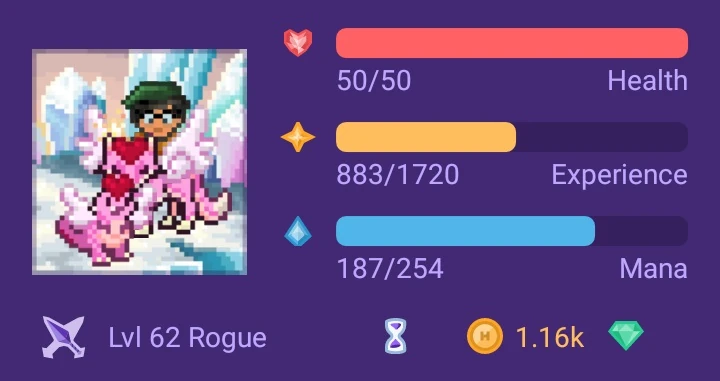
\includegraphics[width=0.7\textwidth]{figures/avatar}
    \caption{Player Avatar in Habitica}
    \label{fig:3}
\end{figure}

\textbf{Curiosity} is a key part of keeping a player interested and engaged with a game. Curiosity is what makes the player want to explore and learn more about the environment and the content of the game and what causes them to keep returning to play again. Games create a sort of second reality for the duration of play, with a set of rules that allows the player to explore and progress within the game, guiding them through the game world \cite{aspects}. The curiosity is triggered and sustained through continuously offering variety and novelty within the game, offering new information, narrative arcs, outcomes and general new elements that keep the player interested and on their toes \cite{engage} \cite{fail}. Offering the player a sense of mystery allows them to tap into their need to get to the bottom of the story or problem at hand, encouraging engagement and an intrinsic sort of motivation \cite{model}.

A recurring element that is found in every game or gamified application out there is \textbf{Challenge}. Challenge is provided through having appropriate levels of difficulty throughout the activity, as well as through progressively more difficult levels or given tasks that let the player work towards previously defined, meaningful goals, encouraging them to put effort into developing strategies and problem-solving to progress within the game \cite{aspects} \cite{engage} \cite{edu} \cite{fail}. The more personal importance the goals have to the player, the more ambition they will have to overcome the challenges given by the application, keeping them motivated \cite{model}. Therefore it is important to be aware of the amount of difficulty that is posed by the challenges. If the activity is too complex and hard to achieve, the player might feel disheartened and lose interest, while on the other hand, if the difficulty level is too low, the player might experience frustration and find the lack of challenge to be demotivating \cite{aspects}.
Especially within a learning context, increasing difficulty is key. Each consecutive task is expected to be more complex than the last, requiring the user to implement their previously gained knowledge and skills to solve the problem at hand \cite{edu}. The addition of new challenges in general is equally a way to coax the user into learning different aspects and new methods of application of the skill or topic they are currently striving to learn \cite{higher}.
Similarly, a game or gamified application should make the required skill \textbf{easy to learn but hard to master}. Through teaching the basics of the required knowledge to tackle the level at hand in simple terms but requiring mastery of this level before being allowed to move to the next, promoting deep engagement with a topic, motivating the user through challenging their understanding of it and rewarding them for successfully integrating the learned knowledge \cite{higher}.
This also fosters \textbf{replayability}, motivating the user to replay and re-engage with the level and the topic until they have proven their learning and understanding enough to progress \cite{fail}. In education and other learning environments, it is crucial to promote a cycle of multiple performances and repetition to allow the student to improve their skills and eventually reach their goal \cite{edu}. Here it is important to actively provide the conditions and opportunities to achieve said goals, using repetition primarily to encourage perseverance after an unsuccessful attempt instead of boring the student with the same subject and not enough new inputs to keep them engaged \cite{edu}. The language learning application Duolingo (developed by Duolingo Inc., 2012) uses a level-oriented system to teach their users, as can be seen in Figure \ref{fig:4} \cite{level}. Through gradual progression and mastery of the levels, the user unlocks the next, while also being allowed to return to previous ones at any time to deepen their skills.

\begin{figure}[h]
    \centering
    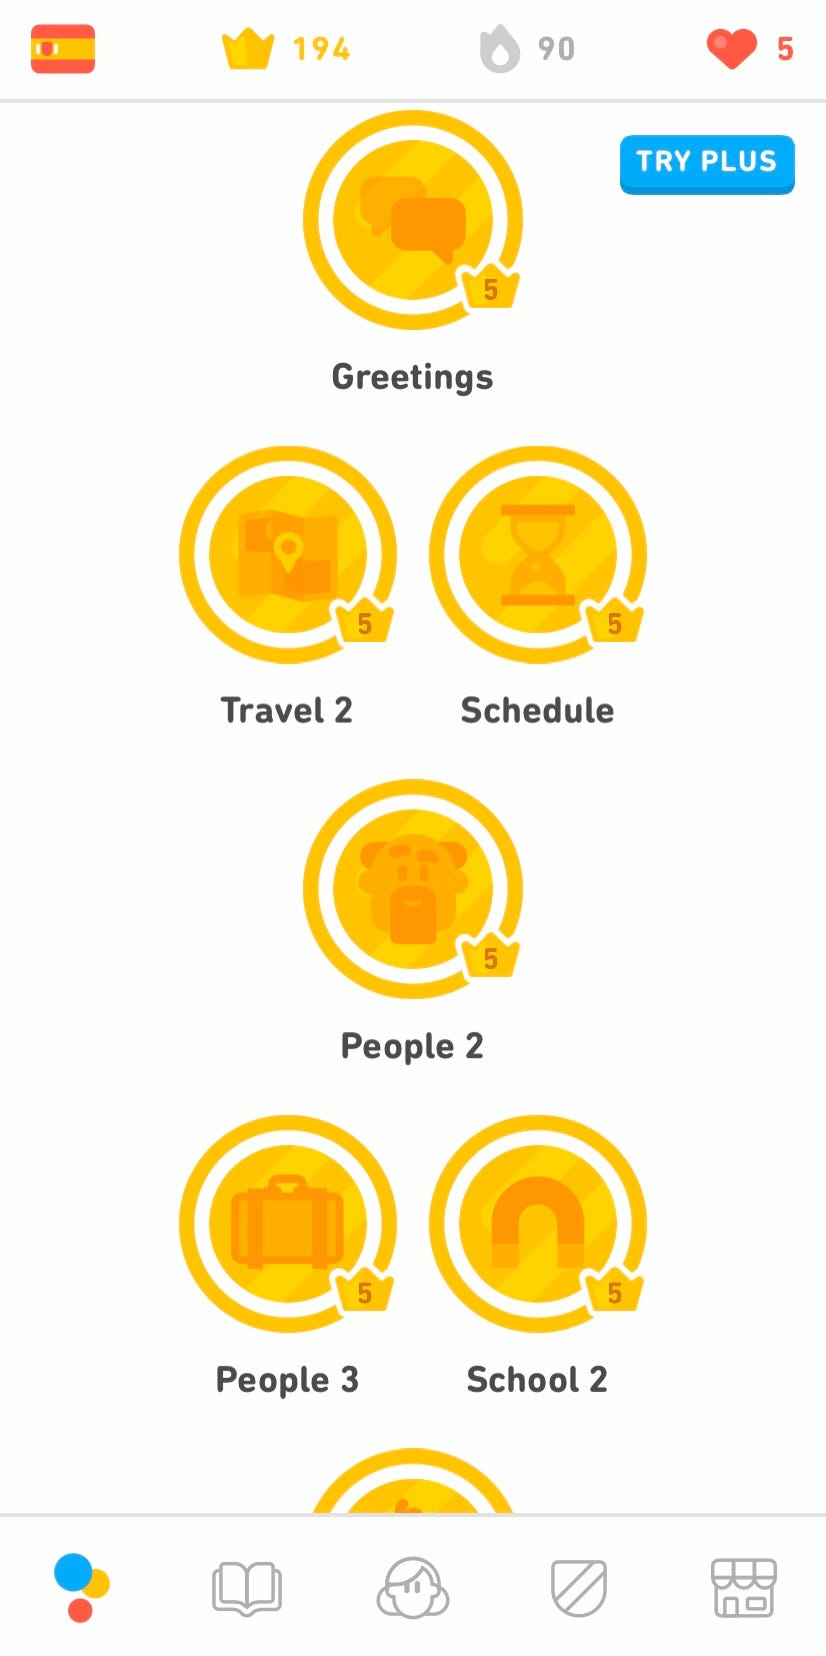
\includegraphics[width=0.37\textwidth]{figures/levels}
    \caption{Level Progression in Duolingo}
    \label{fig:4}
\end{figure}

The probably most important part of any game, gamified tool, or application are the users themselves. All users and players are active participants in the process, not just spectators. This distinctive feature found in all games is equally what plays a key role in gamification \cite{edu}. Inevitably it leads to another main element found in all games and effective learning processes and gamification tools: \textbf{Interactivity}. The more interactive the experience, the more engaging it is \cite{higher}. Interaction means that the players actions trigger events or responses from the application that are related to their immediate manipulations \cite{model}. Another type of interaction that is often present within games is through the affiliations with others. This can be an interaction with a non-player character within a roleplaying game \cite{engage}, or interactions between players, directly or indirectly. This might require direct communication with other players, but is most often used in the form of \textbf{Competition} and \textbf{Collaboration} with others \cite{model} \cite{higher}.
In multiplayer games, collaboration between players can often provide them with a mutual benefit that is very desirable, putting the players who do not play as part of a team at a noticeable disadvantage \cite{lifelong}. This can be through the collaboration within a battle, to the sharing of resources.
While collaboration is a game aspect that some people enjoy, competition usually stays the main motivator and driving force of a game \cite{lifelong}. In a gamified context, competition usually means the comparison of skills, progress and successes to peers and strangers. This can happen in direct confrontation like in the gamified quizzing tool 'Kahoot!' (developed by Kahoot! ASA, 2013) where the participants go head to head in a battle of knowledge, or through comparing in-game statistics like points, badges, their ranking in leaderboards or the amount of achievements in order to gain recognition \cite{higher} or to just feel the satisfaction of having beaten other competitors.

Adjacent to competiton with others is the \textbf{Competition with self}. Through the option to repeat a level for example, the user can compare their performance with their previous try, thereby competing with themselves \cite{fail}. This gives them the possibility to assess their own skill-level and performance, and provides the tools to improve. It is often seen as a very crucial part of any learning process, since the ability to see their own improvements is extremely motivating and rewarding, especially if it is visible in an obvious and continuous manner \cite{lifelong}. Just as in competition with other players, a scoring system can be introduced to visibly keep track of the users progress \cite{lifelong}. A less intrusive way of introducing numbers and visuals to track the individuals progress is for example through experience points or levels.
In the same vein, providing ongoing feedback about their progress and giving general affirmation about the users successes and performance incentivizes them to challenge themselves and perform even better \cite{higher} \cite{engage}.

Generally, users want to feel in \textbf{control} of their own experience and to have the \textbf{choice} and \textbf{freedom} to shape it according to their needs. Control is given to the player by making them feel like their actions have direct and significant concequences \cite{aspects}. This makes them feel valued and empowered and simulates relative freedom of action and freedom of choice, allowing them to move at their prefered pace and doesn't impose on their autonomy \cite{engage} \cite{model}.
A flexibility to select different paths or approaches to the same problem or task can go a long way to make the user feel in control as well \cite{higher}.
Additionally to promoting the feeling of the player being an active part in shaping the process and development of things, the option of \textbf{multiple paths} to reach a goal is fostering the development of a diverse and intersectional skillset, allowing the user to build their own strategies and approaches which is a key characteristic of active learning \cite{edu}.

The \textbf{freedom to fail} is crucial in games, gamification and learning environments alike. This describes the protection from negative concequences for initial failures \cite{engage} which allows the user to explore the topic at their own pace without needing to worry about getting the best results right away, motivating them to seek different approaches to the same task, branching out with their problem-solving skills and gives them the opportunity to thoroughly interact with the subject before moving onto the next one \cite{lifelong}.

Any activity in games and learning should be achievable and reasonable. Especially within an educational environment, the tasks should be adapted to the users pre-existing skill and potential to offer an individual and effective learning experience \cite{edu}. In gamified applications as well, the \textbf{feasibility} of the content is key to provide a positive experience. Through clear communication in the application about what tasks need to be completed and which problems need to be solved \cite{engage}, and through implementing a concise and simple on-boarding process that equally lowers the barrier of entry to start using the application, the process of interaction with the app stays convenient and low effort, which promotes fidelity to using the application regularly, as well as general motivation and feelings of success and progress within the individual \cite{fail}.

Providing \textbf{goals} within the game or learning process is crucial as it dictates the entire content of the application as well as what kind of experience it will be for the user \cite{model}. Users will pursue the goals through interacting with the tasks and problems, gathering the needed items, information, knowledge, etc. that is required to advance within the framework of the game or gamified process. The more focused and clear the goals are, the more engaged the player will be and the easier it will be for them to feel intrinsically motivated \cite{engage}. The goals of the game or application can either be at the end of it, marking the completion of the entirety of the process, or can also be split up into sub-goals that each comprise a topic or task or even just a section of said task to complete. This way, feelings of success can be spread out throughout the entire experience, providing notable rewards or events every time such a goal is reached, fostering ambition and motivation in the user and further creating an effective experience \cite{lifelong}.

Stimulating \textbf{Emotions} and general \textbf{Sensations} of the users is key to providing a satisfying and appealing experience. This refers to the use of visually pleasing graphics within the application, keeping them consistent and simple enough to not overwhelm the user \cite{fail}, as well as to other stimuli for the senses like effective sound design and general appropriate media presentation of the product \cite{model}. Through creating visual or auditive feedback within gamified applications that reward the user after a good performance in a fun and humouristic way, the creation of strong emotions can be stimulated and supported, leading to more engagement, as well as enhance the general enjoyment of the process \cite{fail}.

And last but not least, \textbf{Rewards} are usually the most straightforward and efficient way to foster motivation within the users. Through well thought out rewards that the user considers helpful in their quest to advance within the process, extrinsic motivation can be triggered which usually is a very powerful motivator for many individuals. This ranges from rewards for completing levels, for using the app for multiple days in a row or for getting a new high score \cite{fail}. The most common rewards are elements such as points, badges, achievements or a higher place on a public leaderboard.
The next chapter will dive further into different types of reward systems and different motivators that can be used to keep users engaged.